\chapter{Gravitational waves associated with gamma-ray bursts}

\section{Gamma-ray bursts}

\Acp{GRB} are short, energetic bursts of gamma rays in the MeV range, first discovered in 1967~\citep{Klebesadel_1973}.
Observations throughout the following decades revealed that \acp{GRB} could be classified based on duration and spectral hardness~\citep{Kouveliotou_1993}.
This classification has become the most used to describe \acp{GRB}: long-soft bursts last $\gtrsim2$ s and have soft emission spectra, i.e. lacking in higher energy photons, while short-hard bursts last $\lesssim2$ s and had harder emission spectra.
It is believed that the ultra-relativistic jets required to produce \acp{GRB} come from either black holes~\citep{Woosley_1993} or magnetars~\citep{Dai_1998}.

A multitude of models have been proposed throughout the decades to explain the origins of \acp{GRB}.

Photometry and spectroscopy data provide evidence that long \acp{GRB} originate from \acp{CCSN}, whereas short \acp{GRB} are believed to be associated with compact binary mergers, such as the \ac{BNS} merger GW170817~\citep{gw170817_grb}.

\section{GW searches}

In 2017, the first binary neutron star merger GW170817 was detected by advanced LIGO and Virgo, immediately accompanied by the detection of a relatively low-luminosity gamma-ray burst GRB170817A by Fermi \ac{GBM} two seconds later~\citep{gw170817}.
This prompted a global effort to find an optical, UV, and infrared counterpart that would make up the signature of a kilonova.
The localization provided by the joint detection was sufficient to locate a counterpart near NGC 4993.

\ac{GW} parameter estimation suffers from a degeneracy between distance and orbital plane inclination; increasing the distance of the merger and orienting its orbital plane would both result in a lower \ac{GW} amplitude.
This degeneracy can be broken if either one could be measured externally.
If the joint detection localization were good enough to determine a host galaxy, this would greatly help resolve the distance, however this will more likely require observation of an optical or UV counterpart due to the poor localization provided by current \ac{GRB} and \ac{GW} detectors.
In the case of GW170817, the host galaxy whose redshift was known was used to determine the distance, which then allowed for a more precise measurement of the inclination angle.
A separate analysis using the distance measured from the \ac{GW} detection combined with the known redshift made the first joint \ac{GW}-EM measurement of the Hubble constant, albeit with very large uncertainty due to the small sample size~\citep{gw170817_hubble}.

One of the many unanswered questions surrounding \acp{GRB} pertains to their jet profile, the luminosity as a function of viewing angle (the angle between the observer and the symmetric axis of the jet; the profile is assumed to be axially symmetric and independent of distance).
When information about the jet profile is required, e.g. for making rate estimates for \ac{GRB} detections, the profile is typically modeled as a top-hat (uniform within some opening angle and dropping sharply beyond it) for simplicity, but the true profile may be different.

Determining the viewing angle $\theta_{\mathrm{obs}}$ of a \ac{GRB} is essential for distinguishing between different jet profile models, but it relies on the ability to observe an afterglow emission.
These emissions, ranging from radio to X-rays, follow the prompt emission of $\gamma$-rays and are generated by the interaction between the relativistic outflow and the surrounding medium.
The observation of these afterglows was crucial in improving localization of the \ac{GRB} sources and provided valuable information about the energy scale of the jet, as well as measurements of $\theta_{\mathrm{obs}}$.
The latter came from observing the signature jet break in the afterglow light curve, resulting from the lateral spreading of jet material as it expands; the opening angle can be determined from the timing of the jet break.
However, few jet breaks have been observed for short \acp{GRB}, so existing observations do not place tight constraints on opening angle~\citep{Biscoveanu_2020}.

Joint GW-GRB observations can provide much more information on jet properties~\citep{Mogushi_2019, Farah_2020}.
GRB170817 was orders of magnitude less energetic than most short \acp{GRB}, so it likely would have been ignored in the absence of a \ac{GW} coincidence.
Its low luminosity immediately ruled out an on-axis top-hat jet.
An off-axis top-hat jet was considered unlikely as well because the narrow opening angle predicted for top-hat jets based on theory and past \ac{GRB} measurements only allowed for $\theta_{\mathrm{obs}} \lesssim 10\deg$.
More evidence against an off-axis top-hat model arose when the bright afterglow expected to emerge after $\sim$1 day was not observed.
These observations instead favored a wide-angled, structured jet model for GRB170817.
A structured jet model may refer to any luminosity function that decreases gradually with $\theta_{\mathrm{obs}}$ rather than abruptly, e.g. a Gaussian or power-law with uniform center.
One mechanism that would explain such a model is a cocoon emission, in which the relativistic jet interacts dissipatively with the surrounding merger ejecta, depositing its energy into a cocoon fireball that results in a structured jet~\citep{gw170817_grb}.

\subsection{X-Pipeline}

\section{O3 search for GWs associated with GRBs}

\begin{figure}[h]
  \centering
  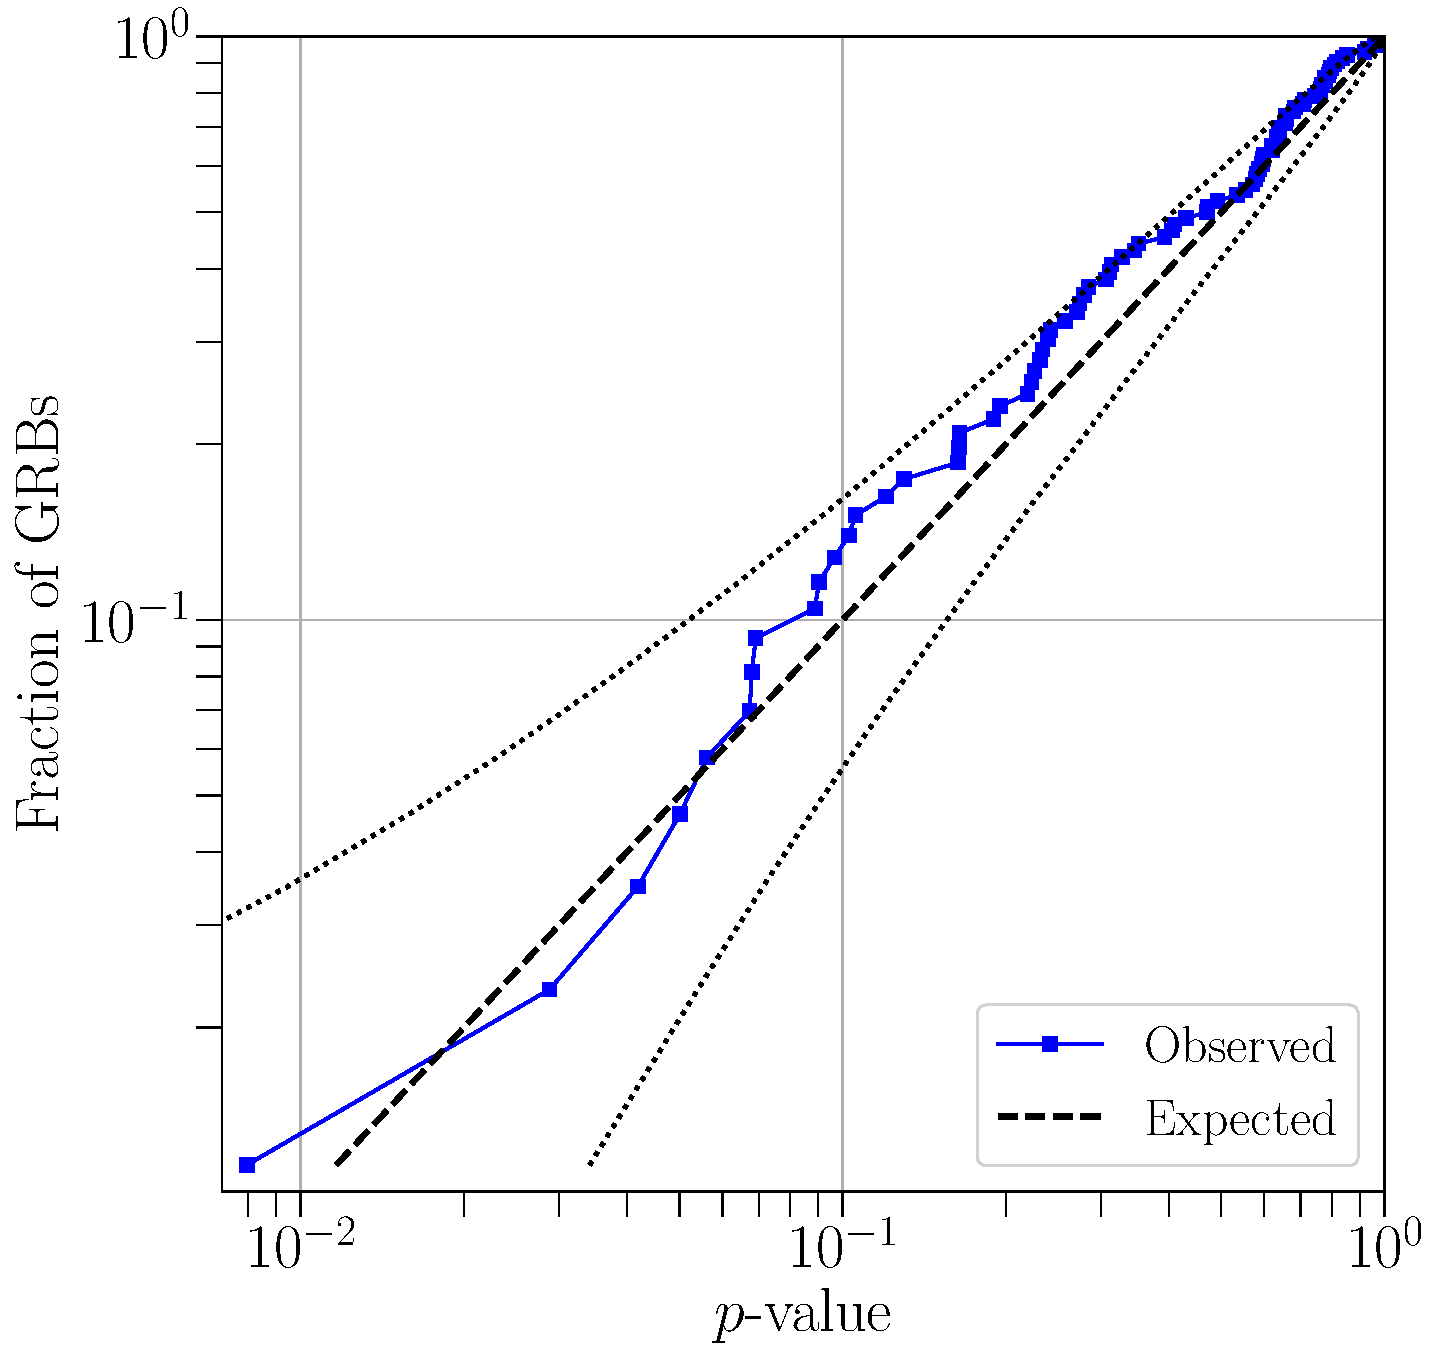
\includegraphics[width=0.7\textwidth]{figures/grb/o3b-x-pval.pdf}
  \caption{P-values of O3b X-pipeline analyses.}
  \label{fig:grb-o3b-x-pval}
\end{figure}

\begin{figure}[h]
  \centering
  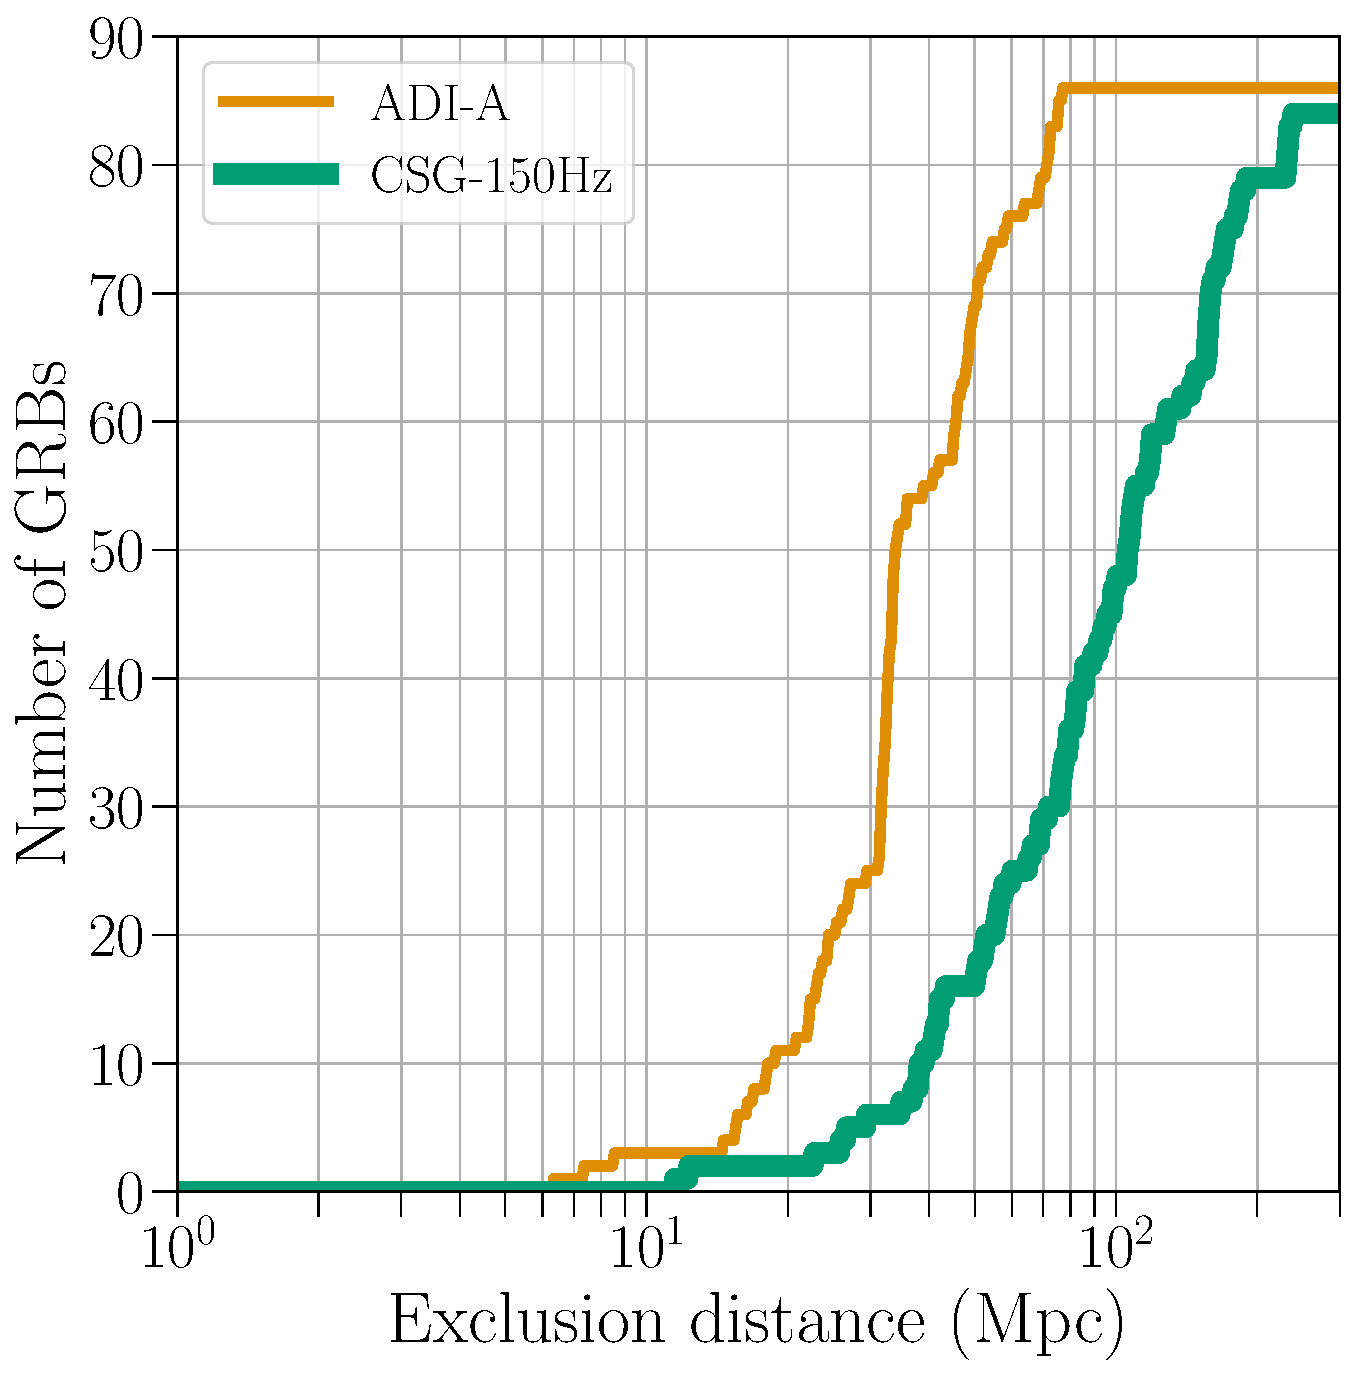
\includegraphics[width=0.7\textwidth]{figures/grb/o3b-x-exclusion.pdf}
  \caption{Cumulative distribution of O3b X-pipeline exclusion distances for 150-Hz sine-Gaussian and ADI-A waveforms.}
  \label{fig:grb-o3b-x-exclusion}
\end{figure}

\subsection{GRB sample}

\subsection{Results}

\subsection{Noise assessment}
